 \mysection{The Pooka}{species-pooka}

  \flavor{In the mists before the Beginning, Fate and Chance cast lots to decide whose the game should be; and he that won strode through the mists to \TheAuthority and said: "Now make Gods for Me, for I have won the cast and the Game is to be Mine."  Who it was that won the cast, and whether it was Fate or whether Chance that went through the mists before the Beginning to \TheAuthority - none knoweth. \Tilde Lord Dunsany, \myital{The Gods of Pegana}}


\begin{center}
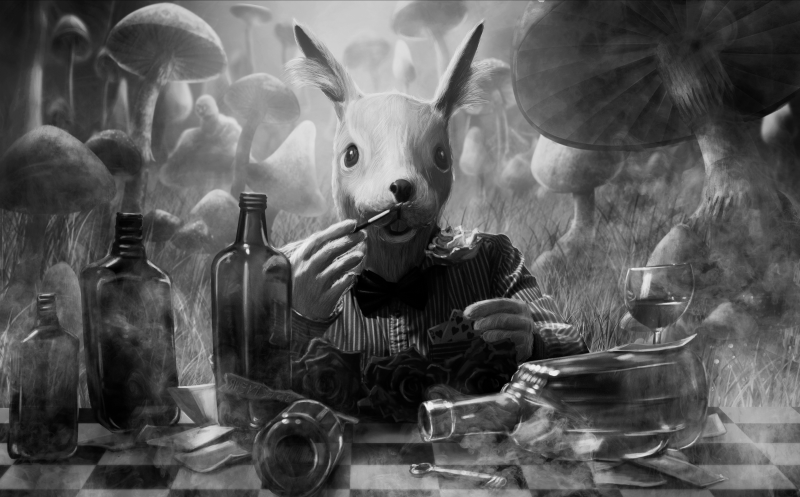
\includegraphics[width=\linewidth,keepaspectratio=true]{species/Pooka1}
\end{center}



\begin{multicols*}{2}\raggedcolumns

  \mysubsection{Appearance}{pooka-appearance}
    
  You do not believe in Fate - it's a made up idea, created by people who are terrified that we are plunging headlong through the void with no rhyme or reason.  Chance and Chaos govern the Totality.  This is reprehensible to \TheAuthority, who seeks to keep the secret of the game of lots from us.  But you are proof that it is Chance that was victorious, and for this you are cursed, and marked Unhallowed.

    While you aren't the social pariahs that the Rom (Murks and Spriggans) are, Mortals don't fully trust you.  Most Mortals will refuse to play games of chance with you; they won't loan or give you money if they can help it ("he'll just put it up his nose!"); and they won't direct questions to you if there are other Mortals in your Band present.

  You stand scarcely 1m tall, with the head and feet of a rabbit, pig, goat, or toad.  You are gregarious, sly, and always at the point of laughing.  Pooka love to be around people, and it's not uncommon to find them on ships (where they're thought to be good luck), tending bars (if they don't drink away their profits), or with gypsy troupes.  You excel at dancing and singing, and take every opportunity to do both.




\newpage

  \mysubsection{Creation}{pooka-creation}

  Write down the following information on your \mylink{Adventurer Sheet}{adventurer-sheet.9}

  \callout {
    \mynumlist {
        \item You start with \mybold{2 Flesh and 8 Grit}.
        \item Move your \PRE \DCUP (to a d6).
        \item If you need to \RSTRY{\PRE}, you only fail on a natural 1 (instead of a 1 or 2). Put a check next to \PRE on your Adventurer Sheet so you don't forget.
        \item You are lucky to have around. You have a d4 \mylink{Lucky Die}{pooka-lucky-die}.
        \item Write down your \mylink{Virtues}{pooka-virtues}.
        \item Write down your \mylink{Complication}{pooka-complications}.
        \item Write down your \mylink{Starting Gear}{pooka-starting-gear}.
    }
 }



  \myhighlight{Lucky Die}{pooka-lucky-die}

  Your Lucky Die is a Resource Die whose result can be applied to \mybold{someone else's} \RO or \RB try (either in or out of Combat). You may roll this \UD and add it to the result. You can only use this roll to help a member of your Band, and no one else (including yourself). You can roll your Lucky Die \myital{after} the person attempts their try (it doesn't have to be at the same time), but you can only add a single roll to their total.

\mybold{Your Lucky Die starts as \UDD{d4}}. Your Lucky Die moves \DCDOWN on Failure.

\begin{center}
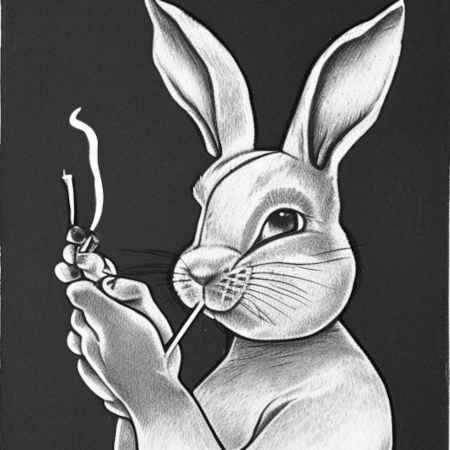
\includegraphics{species/Pooka2}
\end{center}

    \mysubsection{Virtues}{pooka-virtues}

    \myhighlight{Apotropaic}{pooka-virtue-apotropaic}
  
    Your very presence wards off evil:

    \mybullet {
        \item Buildings where you are sleeping are protected from casual attack (meaning the building would be spared in a riot, for example).  
        \item \mypg{Wandering Monsters}{arbiter-monsters-wandering} will bypass your camp.
        \item The members of your Band are immune to the effects of a \mypg{Jinx Charm}{charm-jinx}.
        \item You are immune to \mypg{Curses}{cunning-curses}, including those invoked by a \mypg{Malison}{occultism-malison}.
    }



    \myhighlight{Bro, Hit This}{pooka-virtue-hit-this}

    For any \mypg{Narcotics}{gear-narcotics} you take, the \UD only moves \DCDOWN if you roll a 1, and you only Fail an \mylink{Addiction}{gear-narcotics-addiction} or \mylink{Overdose}{gear-narcotics-overdose} try on a 1 (instead of a 1 or 2).  When you take a \mylink{Downtime}{downtime}, \RS using your Luck die; if you don't Fail, you can obtain \UDD{d4} of \myital{any} \mylink{Common Narcotic}{gear-narcotics} for free (even Narcotics that would normally not be available, like Black Lotus in a Small settlement).
    

\myhighlight{Curious}{pooka-curious}

Gain are Untrained (1) in the \mylink{Whispers of Br'er Rabbit}{vulgate-whisper-brer-rabbit}. See the section on \mypg{Whispers}{vulgate-whisper-brer-rabbit} for more info.


    \myhighlight{Hype Man}{pooka-virtue-hype-man}

    If you take a \mylink{Breather}{combat-resting-breather}, roll a d4 for each member of your Band (including yourself). You can restore \SUM points of Grit to yourself or any other members of your Band (you get to decide how this is divvied up).  Additionally, if you \mypg{help out}{skills-helping-out} someone with a Skill, you don't count towards the "only one person can help" rule.

\newpage

\myhighlight{Just What I Needed}{pooka-just-needed}

Once per Session, you may pull one of the following out of ... someplace ... on your person:  a) \UDD{d4} of \mylink{Smokes}{gear-narcotics-smokes}, b) \UDD{d4} of \mylink{Alcohol}{gear-narcotics-alcohol}, c) d4\AG coins, d) \UDD{d4} of \mylink{Provisions}{gear-equipment}. If you don't use what you produced before the end of the Session, they disappear (food was just about to turn, you lose the coins, etc.)

  \myhighlight{Undreamt}{pooka-virtue-undreamt}

  You stand outside of the Dream and are thus untouched by Sish, the Handmaiden of Time. You are immune to aging of any kind, and your \DEATH starts at Tough (d4).


  \myhighlight{We're All Mad Here}{pooka-madness}

   If you roll a Failure when attempting an \mylink{Insanity}{adventurer-kismet-insanity} try, you only suffer negative effects if you're "mind breaks" (that is, if you roll a 10 and must therefore roll on the \mylink{Madness!}{injury-insanity-madness} table).



    \myhighlight{Wired}{pooka-virtue-wired}
  
    No one can get the \mylink{Drop}{combat-drop} on you, you always win \mylink{Init}{combat-init} (no need to roll), and you are immune to: \effect{Charmed} and \effect{Slept}.


    \mysubsection{Complications}{pooka-complications}

    \myhighlight{Distrusted}{pooka-complication-Distrusted}

  Any time you stay in a Tiny \mylink{Settlement}{civilization-settlements}, you run the risk of being accused of something by the superstitious.  If you stay in a \mylink{Tiny}{civilization-settlements} thorp, dorf, etc. roll 2d6 - on a 2 (snake-eyes) you're accosted for poisoning the well water / getting the farmer's daughter pregnant (your gender is irrelevant) / making the chickens sick, etc. If you roll a 12 (boxcars), you'll be called on to do something important - deliver a baby, heal someone's fever, etc. - should you fail, the consequences can be dire.

\cbreak

    \myhighlight{Tiny}{pooka-complication-tiny}

  You stand only 1m tall to start.  You can only carry a \mylink{Burden}{gear-burden} equal to your \VIG (you don't get the +2 bonus). If you wear armor, you can only wear armor for "little people" (child-sized).  You cannot wield 2-handed weapons.

  \myhighlight{Unseelie}{pooka-complication-unseelie}
    
  You are creature of Chaos, one of the \mylink{Unseelie}{the-inhabitants} - and are thus \mybold{Unhallowed}.


  \mysubsection{Starting Gear}{pooka-starting-gear}

\callout{\footnotesize{
  You begin with:

  \mybullet {
    \item 1 gold piece; 
    \item two iron \mylink{Daggers}{gear-dex-weapons} or a \mylink{Throwing Axe}{gear-vig-weapons};
    \item \UDD{d4} of \mylink{Personal Provisions}{gear-equipment};
    \item \UDD{d4} of a \mylink{Narcotic}{gear-narcotics} of your choice;
    \item 5 rolls on the \mylink{Random Items}{appendix-a-random-items} table in Appendix A;
    \item playing cards or dice
  }}}


 
    \myhighlight{What Next?}{pooka-what-next}

    Pooka are physically very weak, so they need to "augment" themselves as much as possible. Take a look at \mypg{Narcotics}{gear-narcotics} and the \mypg{Whispers of Br'er Rabbit}{vulgate-whisper-brer-rabbit}. You're one of the best ways for a Band to heal Grit, so make sure you understand how taking a \mypg{Breather}{combat-resting-breather} works, as well.


\end{multicols*}
